In \Cref{sec:hebbian-kernel-mlps}, we characterized the margin scaling of \emph{Hebbian MLPs}. In this section we leverage our margin scaling bounds to study the storage capacity scaling of Transformer blocks, where MLP inputs are no longer exact keys but instead are noisy attention outputs. Crucially, we demonstrate that the fact storage capacity of Transformer blocks scales at the information-theoretically optimal rate, provided the attention noise remains bounded. Further, we empirically show that our construction remains usable within Transformer blocks for factual recall tasks; at matched fact count, the NTK baseline requires roughly $15$-$63\times$ more parameters than Transformer blocks using our data-dependent construction. Finally, we show that fact-storing MLPs unlock a new capability: modular, zero-shot fact editing within a Transformer by \emph{swapping out its MLP}.

\begin{figure*}[t]
\centering
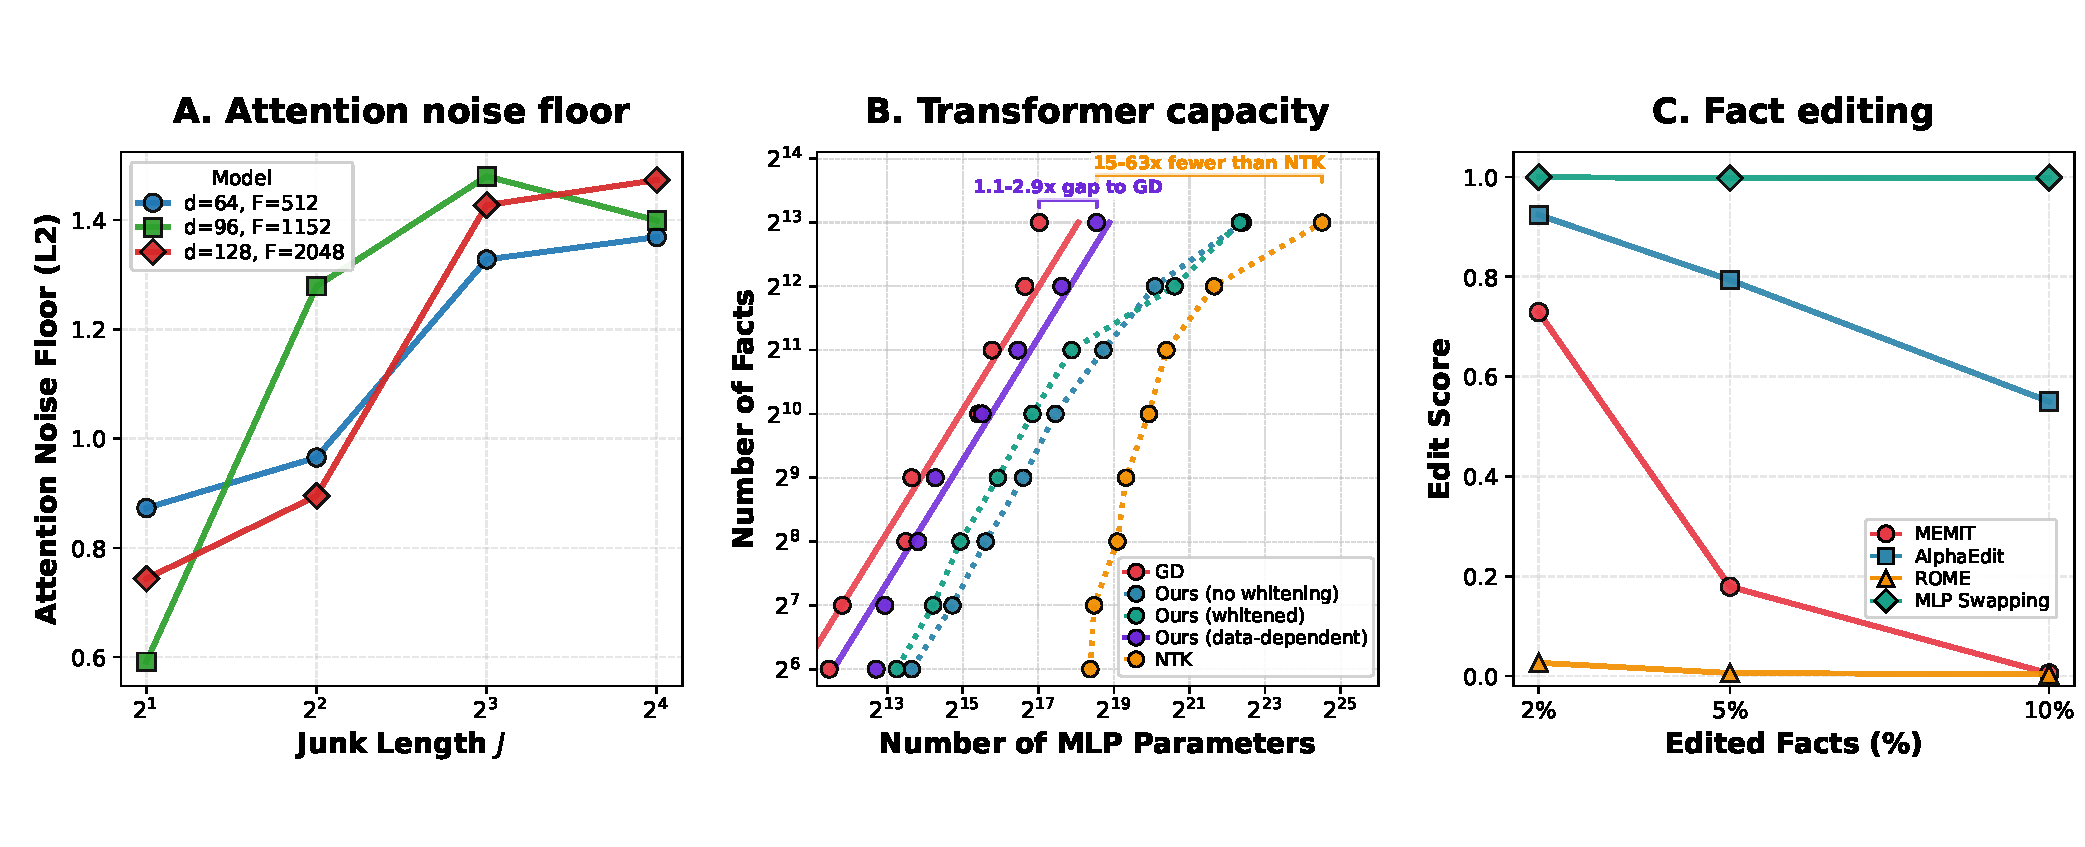
\includegraphics[width=\linewidth]{sections/section_5_transformer_integration/figs/fig3_transformer_integration_1x3_labeled_titled_review.pdf}
\caption{\textbf{Transformer blocks achieve information-theoretic optimal fact-storage capacity and enable modular fact editing.}
\textit{(A)} Attention noise ceiling $\varepsilon_{\mathrm{attn}}$ scales with junk context length $J$ in SSFR.
\textit{(B)} Under bounded attention noise, Transformer blocks with our MLP construction achieve information-theoretic optimal fact-storage capacity scaling.
\textit{(C)} \textsc{MLP Swapping} achieves near-perfect fact-editing score ($>\!0.99$) at up to $10\%$ edited facts, more than 40\% better than existing fact-editing baselines.
}
\label{fig:ssfr_main_fig}
\end{figure*}

\subsection{MLPs in Transformers Achieve Optimal Fact-Storage Capacity}
\label{subsec:transformer-capacity}
\label{subsec:attention-noise}

We start by investigating why MLPs need positive margin in Transformers.
Unlike in the standalone setting, attention does not query the MLP with the exact stored key.  We quantify the worst-case deviation formally with an \emph{attention noise ceiling}, which we define as the maximum noise an attention layer can produce when querying an MLP for a fact:

\begin{definition}[Attention noise ceiling -- informal]
\label{def:attn-noise}
Let $Q_i \subset \mathbb{R}^d$ be the set of all possible queries an attention layer can produce when querying the MLP for the fact corresponding to the key $\mathbf{k}_i$. The \emph{attention noise ceiling} is defined as
\[
  \varepsilon_{\mathrm{attn}}
  := \max_{i \in [F]}\; \max_{\mathbf{q}\in Q_i} \|\mathbf{q} - \mathbf{k}_{i}\|_{2}.
\]
\end{definition}


Intuitively, we find that the attention noise ceiling increases with the number of distractor tokens in the sequence being processed by a Transformer block (Figure~\ref{fig:ssfr_main_fig}). We next show that Transformer usability reduces to whether the MLP margin can handle perturbations at this scale.





\paragraph{MLPs achieve optimal fact-storage capacity in Transformers.}
We now present our main result. Equipped with our margin scaling analysis in MLPs, we demonstrate that Transformer blocks can store facts at an information-theoretic optimal rate, provided bounded attention noise ceiling:

\begin{tcolorbox}[breakable,colback=white,colframe=blue!50!black,boxrule=1.5pt,arc=0mm,left=8pt,right=8pt,top=8pt,bottom=8pt,title={\small\bfseries Key Result: Transformer blocks can store facts at an info-theory optimal rate.},colbacktitle=blue!50!black,coltitle=white,titlerule=0.5pt]
\begin{theorem}[Transformer Block Fact-storage Capacity (Isotropic Embeddings) - Informal]
\label{thm:noise-robust-capacity}
A Transformer block equipped with a fact-storing bilinear MLP, with non-trivial margin $\gamma_{\min}>c_0>0$, for constant $c_0$, can store $F$ facts using
\[
  W = \Theta(md)
    = \Theta\!\left(F\log (F)\right)
\]
MLP parameters, provided the attention layer in the block satisfies the \textit{attention noise ceiling}
\begin{equation}
  \varepsilon_{\mathrm{attn}}
  \lesssim
  \frac{c_0}
  {L_{\mathrm{bil}}\!\left(
    \sqrt{\frac{F\log(F)}{d}}
  \right)} .
  \label{eq:eps-cap}
\end{equation}
where $L_{\mathrm{bil}}$ is the Lipschitz constant of the MLP. 
\end{theorem} See Appendix~\ref{app:theory:transformers_perturbation} for formal statement and proof.
\end{tcolorbox}
\Cref{cor:capacity-new} presents the formal statement and proof. We note that this result can be easily extended to arbitrary embedding geometries, incurring the same penalization factors from \cref{eq:maintext:akav_margin_bound}.

\paragraph{Empirical verification.}
We produce GD, NTK, and our constructed MLPs, freeze their parameters, then insert them into a 1-layer Transformer and train on the SSFR task.
Figure~\ref{fig:ssfr_main_fig}b validates the predicted asymptotically optimal capacity scaling for Transformer blocks using our construction.
Appendix~\ref{app:theory:transformers_perturbation} reports a complementary per-key margin diagnostic; in particular, \Cref{fig:margin-violin} shows that the usable-key fraction inferred from per-key margins closely tracks end-to-end Transformer accuracy.
Among the constructions we evaluate, our data-dependent construction only requires at most $3\times$ more parameters than GD MLPs at matched fact count. Relative to the NTK baseline, our data-dependent construction requires $15$-$63\times$ fewer parameters at matched fact count. See Appendix~\ref{app:theory:transformers_perturbation} for further diagnostics.



\subsection{Fact Editing via \textsc{MLP Swapping}}
\label{sec:fact-editing}

Having demonstrated that fact-storing MLPs are usable inside Transformers, we now use GD-trained fact-storing MLPs to show a simple proof-of-concept method for \emph{zero-shot fact editing}. We call this procedure \textsc{MLP Swapping}: to edit the model's facts, we construct a new MLP storing the revised fact set and swap it into the Transformer, with \emph{no further tuning of the Transformer's parameters}.

We evaluate on a synthetic author-book language-modeling task (Appendix~\ref{appendix:fact-editing}) using a one-layer Transformer trained to store book--author facts through a frozen fact-storing MLP.
After training, we edit a subset of stored facts and evaluate two metrics. The first is the standard fact-editing score~\citep{memit}, which jointly captures edit efficacy (edited facts predict the new values), specificity (unedited facts stay correct), and paraphrase generalization (edits transfer to paraphrased prompts). The second is the non-fact PPL ratio, measuring post-edit versus pre-edit perplexity on non-fact tokens.
\textsc{MLP Swapping} achieves near-perfect fact-editing score across the edit fractions we test.
At $10\%$ edited facts, \textsc{MLP Swapping} achieves score $0.999$---a $44.9$-percentage-point gain over the strongest baseline, AlphaEdit~\citep{fang2025alphaeditnullspaceconstrainedknowledge} (score $0.550$)---while achieving a non-fact PPL ratio of only $1.02$ (Figure~\ref{fig:ssfr_main_fig}c).

Appendix~\ref{appendix:fact-editing} further shows that \textsc{MLP Swapping} also works for a data-dependent constructed Hebbian MLP.
\textsc{MLP Swapping} with Hebbian MLPs keeps the edit score above \(0.98\) through up to \(10\%\) edited facts, while the strongest baseline reaches only \(0.847\)---a 13.3-percentage-point gain (Figure~\ref{fig:fact-editing-constructed-data-dependent}).
